% !TeX spellcheck = es_ES 
\documentclass{article}
\usepackage[section]{placeins}
\usepackage{enumerate}
\usepackage{makecell} 
\usepackage{graphicx}
\usepackage{url}
\usepackage[spanish]{babel}
\usepackage[utf8]{inputenc}
\usepackage[backend=biber, style=numeric]{biblatex}
\addbibresource{ProtocoloRSL.bib}

\begin{document}
  \title{%
  Protocolo de investigación\\

  \large Revisión de la literatura sobre las actividades de requisitos para Software como Servicio\\}
  \author{Alberto de Jesús Sánchez López \\ 
  \small Proyecto Guiado}
  \author{\makebox[.9\textwidth]{Alberto de Jesús Sánchez López }\\Universidad Veracruzana \and M.C.C.María Angélica Cerdán \and Dr.Jorge Octavio Ocharán Hernández}
  \author{\makebox[.6\textwidth]{Alberto de Jesús Sánchez López}\\Universidad Veracruzana\\ \and M.C.C. María Angélica Cerdán \and Dr. Jorge Octavio Ocharán Hernández}
  \date{07 de enero del 2021}
  \maketitle
  \hfill
  \begin{tabular}{@{}p{.5in}p{4in}@{}}
          Versión final: & \hrulefill \\
          & M.C.C María Angélica Cerdán \\
  \end{tabular}
  \thispagestyle{empty}
  \newpage

  \tableofcontents
  \thispagestyle{empty}
  \newpage

\setcounter{page}{1}
\section{Antecedentes}

El concepto de rentar recursos computacionales como servicio, fue introducido en 1971 a la industria por IBM (de sus siglas en inglés International Business Machine) y RJE, empresa de manufactura de microprocesadores que 
trabajaba para IBM. En aquel momento, el término se denominó “time-sharing” \cite{antecedentes6}. Con el transcurrir del tiempo, la adopción de esta modalidad de distribución ha provocado un cambio importante en la forma 
de adquisición de bienes en Internet, motivando el surgimiento de proveedores en servicios digitales dinámicos, que proveen funcionalidades y modelos de pago flexibles, así como un proceso de adquisición totalmente 
automático (autoservicio), donde la disposición del recurso debe ser ejecutada, otorgada y administrada en su totalidad en línea.

A este modelo aplicado al software, se le llama SaaS (por sus siglas en inglés Software as a Service), que ha sido ampliamente adoptado debido a que permite una economía de escala en el desarrollo de software y al nivel 
de acceso que permite un modelo que se ejecuta en la nube, lo que hace conveniente la adquisición bajo este formato. Dentro del primer trimestre del año en curso, se observó un crecimiento del 30%
en el porcentaje promedio de ventas anuales, producido por aplicaciones SaaS de tipo empresarial en el mercado global, según Microsoft \cite{antecedentes7}. Otro estudio revela que algunos de los factores más influyentes en el 
proceso de adopción de software como servicio, es el manejo de seguridad y privacidad de los datos, la ventaja competitiva de adquirir software que ha pasado bajo un proceso de validación, así como una adopción de cultura orientada a la comunicación.

La tendencia a adoptar trabajo en casa y educación línea, causado por la pandemia, ocasionada por el virus Sars-COV2, motivará un crecimiento en el desarrollo de aplicaciones orientadas al SaaS \cite{antecedentes5}. Esto hace 
surgir una necesidad a aquellos interesados sobre la información relacionada al desarrollo de un Software como Servicio.
Como todo proceso de desarrollo de un sistema de software, no es una actividad sencilla, sigue las fases convencionales reconocidas en el campo de la Ingeniería de Software y puede aplicar estándares internacionales 
que definen el ciclo de vida del software, sin embargo, este tipo de aplicaciones enfrentan condiciones relativas a su propia naturaleza, que motivan la adaptación de los procesos básicos pertenecientes al desarrollo de software 
tradicional, así como el estudio de los métodos que se utilizan dentro del mismo.

Un área de especial interés, es la definición y administración de requisitos, un requisito es determinado como “Descripciones de los servicios que un sistema debería proveer y las restricciones en su operación… El proceso de encontrar, analizar, 
documentar y verificar los servicios y restricciones de un sistema es llamado Ingeniería de requisitos” según \cite{antecedentes8}. Es decir, la fase de definición de requisitos es un proceso complejo y con gran importancia en el ciclo 
de vida de un producto de software, puesto que una definición detallada de los requisitos influye en la calidad del producto final, por ende, la especificación de los requisitos, debe ser un artefacto producido mediante un 
proceso bien delimitado, planeado, probado y medido. Si la especificación de requisitos ha sido resultado de un proceso formal, la probabilidad de que el proyecto sea un éxito, aumenta \cite{antecedentes}.

Para llevar a cabo un proceso de desarrollo de software que asegure calidad en el producto final, es importante una fase de definición de requisitos de software sólida \cite{antecedentes4}, años de investigación y 
experiencia recabada por la comunidad, ha hecho que el desarrollo de requisitos para sistemas tradicionales sea un tema basto en información, lo que facilita el proceso de planeación de una elicitación.

Pero la definición de requisitos para un Software como Servicio, está muy lejos de ser tradicional \cite{antecedentes1}, en esta área relativamente nueva, es fundamental analizar la 
información disponible relacionada al tema y plantear una propuesta que se apegue a las necesidades especiales del desarrollo de un software como servicio. 

Definir un proceso para recolectar información sobre las actividades y metodologías utilizadas en el contexto actual de desarrollo de requisitos en un software como servicio, no es una tarea sencilla, debido a que la información existe, 
pero está dispersa, no hay una compilación formal sobre la misma. Esto es de gran interés para aquellos investigadores interesados 
en sistemas en los que existe una necesidad general a cubrir o un conjunto de clientes con una necesidad en común, pero con requisitos individuales específicos, se presentan complejidades que necesitan atención especial. 
 
Esto genera una oportunidad para disminuir la brecha de conocimiento dentro del área, por medio de una Revisión Sistemática de la Literatura que documente el estado del arte sobre las actividades y metodologías identificadas
en la fase de requisitos para el Software como Servicio, la cual proveerá punto de inicio para aquellos interesados en el estado actual de las actividades de requisitos realizadas para un software como servicio. 
\newpage

\section{Planteamiento del Problema}
Con la adopción del software como servicio en la industria y la necesidad creciente de documentar los procesos relacionados al mismo, se presenta la oportunidad para investigar y documentar las actividades 
relacionadas con su elaboración, en este caso, de la fase de requisitos, un elemento clave para asegurar la calidad de cualquier 
producto de software según \cite{antecedentes}. Actualmente no existen recopilaciones formales dirigidas a las actividades de requisitos para un Software como Servicio, existe información disponible, 
pero está dispersa, no está enfocada en un software como servicio y no existe una compilación sobre el estado del arte en actividades o métodos existentes, esto provoca la falta de dirección 
clara para investigaciones en el área. Por lo que, el problema que motiva el presente trabajo se puede enunciar de la siguiente forma:\\

\textbf{No existe un análisis sobre el estado del arte sobre las actividades realizadas dentro del proceso de requisitos en un Software como Servicio.}\\

Lo anterior es un obstáculo para aquellos investigadores interesados en iniciar estudios enfocados a actividades de requisitos para un software como servicio, 
esto causa cierta urgencia, ya que para realizar investigaciones enfocadas a las actividades (evaluación, mejoras, clasificar) es necesario, identificar el estado actual de las mismas, no existe tal 
investigación actualmente.


\newpage

\section{Objetivos}
\textbf{Objetivo general} \\

Analizar el estado del arte sobre el proceso de requisitos en el desarrollo de Software como servicio a través de una revisión sistemática de literatura, para identificar temas abiertos en el área disciplinar. \\

\textbf{Objetivos específicos} \\

\begin{itemize}
    \item Establecer las preguntas de investigación que permitan analizar el estado del arte sobre el proceso de requisitos en el desarrollo de software como servicio, que deberán ser respondidas por la revisión sistemática de literatura.
    \item Realizar una búsqueda de literatura especializada en bases de datos confiables, aplicando criterios de inclusión y de exclusión para determinar los documentos a analizar.
    \item Extraer información relevante de los documentos seleccionados de la literatura especializada, a través de una matriz de extracción que permita el análisis de métodos y técnicas aplicadas en el proceso de requisitos en el desarrollo de software como servicio.
    \item Aplicar una técnica de metaanálisis para contrastar y combinar las propuestas de los diferentes estudios contenidos en la literatura especializada para el proceso de requisitos en el desarrollo de software como servicio.
    \item Identificar las tendencias en las propuestas analizadas de la literatura especializada para determinar los temas abiertos en el área disciplinar de los procesos de requisitos en el desarrollo de software como servicio.
\end{itemize}

\newpage

\section{Justificación}

Actualmente, no existe una revisión formal sobre la Literatura dirigida hacia identificar el estado estado del arte sobre las actividades de requisitos realizadas para un Software como Servicio, 
Realizar un análisis sobre las actividades y metodologías involucradas en el desarrollo de requisitos para un software como servicio, sería de gran ayuda para documentar la visión general de las actividades 
empleadas para elicitar, analizar y validar los requisitos, una investigación de esta naturaleza, permitiría iniciar estudios enfocados a evaluar, analizar y mejorar las actividades 
identificadas, lo cual propone un conjunto de investigaciones para trabajos futuros.

Realizar la Revisión Sistemática de Literatura permitiría lo siguiente: 

\begin{itemize}
    \item Desarrollar una compilación formal sobre el estado de arte actual de las actividades de requisitos llevadas a cabo en un software como servicio.
    \item Documentar las actividades empleadas para la elicitación, análisis y validación de requisitos para un software como servicio.
    \item Documentar las áreas de investigación propuestas  en el área de requisitos en el software como servicio.
    \item Proponer áreas de investigación potenciales en el área de requisitos en el software como servicio.
\end{itemize}
\newpage

\section{Alcances y Limitaciones}
\textbf{Alcances} \\
Se realizará una revisión sistemática de la literatura para documentar el estado actual de las actividades 
empleadas en el proceso de requisitos para un software como servicio, con el fin de establecer una vista 
actual sobre las actividades realizadas para la elicitación, los retos encontrados, así como también
documentar las actividades relacionadas con el análisis y validación de requisitos para un software como servicio. 

\textbf{Limitaciones} \\
No se pretende desarrollar una guía para llevar a cabo un proceso de requisitos en un software como servicio, el trabajo 
proporcionará un análisis sobre el estado actual de las actividades y metodologías utilizadas en la fase de requisitos, que han sido 
documentadas en la literatura, enfocándose en estudios primarios como fundamento principal para la revisión sistemática. 
\newpage

\section{Método}
Se utilizará una revisión sistemática de la literatura para llevar a cabo esta investigación, 
empleando la guía \cite{metodo}. Donde se especifican preguntas de investigación que tienen 
como objetivo dirigir la investigación, después se emplea una una búsqueda manual como estrategia de búsqueda y 
se aplican criterios para la inclusión y exclusión de estudios, terminando el proceso con una síntesis de la información 
recabada, utlizando la guía enfocada a síntesis narrativa, siguiendo la guía \cite{sintesisnarrativa}.

\begin{figure}[!htb]
   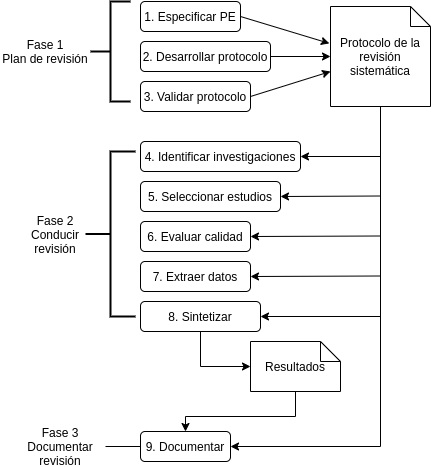
\includegraphics[width=\linewidth]{metodo.png}
   \caption{Visión general del método para la revisión sistemática de la literatura.}
   \label{fig:etapasconducción}
\end{figure}

\newpage

\section{Cronograma}
Se diseñó un cronograma, que contiene el conjunto de actividades clave para completar la revisión sistemática de la literatura, 
con el propósito de determinar tiempos de ejecución, documentar las tareas a llevar a cabo y asignar espacios de tiempo apropiados 
para completar la revisión en el periodo designado. Para realizar lo anterior es necesario calcular las horas necesarias para completar el proyecto. 
La formula utilizada para calcular el total de trabajo, fué extraído del manual "Manual para la presentación de anteproyectos e informes de investigación" \cite{manualcronograma}.
Se llegó a un total de 373 horas, las cuales fueron asignadas entre los días de de trabajo del periodo escolar actual, el cual contiene 120 días.
Se planeó un promedio de tres horas diarias de trabajo en el transcurso del periodo. 

\begin{figure}[!htb]
   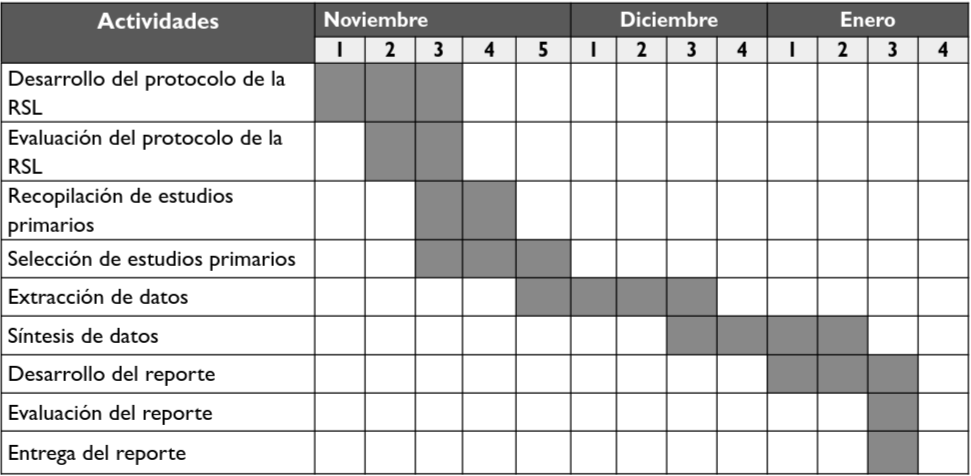
\includegraphics[width=\linewidth]{gant.png}
   \caption{Cronograma de actividades.}
   \label{fig:etapasconducción}
\end{figure}

\newpage

\section{Referencias}
\printbibliography

\end{document}
